\documentclass[11pt, oneside]{article} 
\usepackage{geometry}
\geometry{letterpaper} 
\usepackage{graphicx}
	
\usepackage{amssymb}
\usepackage{amsmath}
\usepackage{parskip}
\usepackage{color}
\usepackage{hyperref}

\graphicspath{{/Users/telliott_admin/Tex/png/}}
% \begin{center} 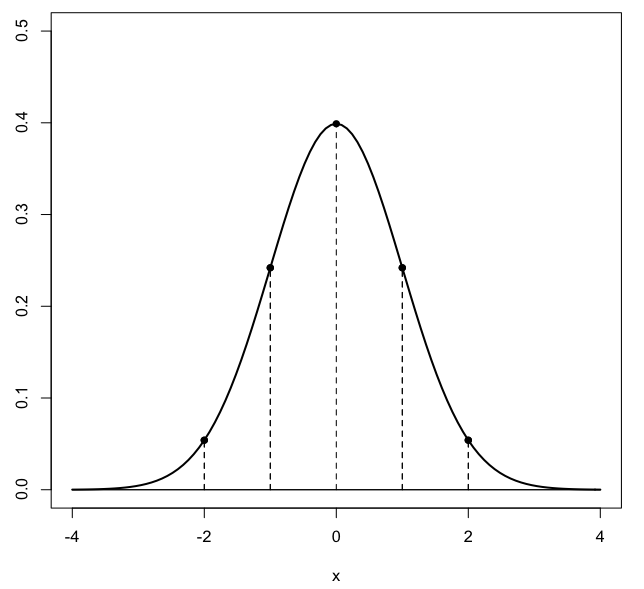
\includegraphics [scale=0.4] {gauss3.png} \end{center}

\title{Volume of the sphere}
\date{}

\begin{document}
\maketitle
\Large


\label{sec:Volume_of_the_sphere}

This chapter is mainly review.  We look again at the problem with which we started the book, finding the volume contained inside a sphere.  

Officially, the sphere is the set of points at a specified distance $R$ from the origin (i.e., it's hollow), and the volume inside is technically called a "ball".  But we'll just use the phrase "volume of the sphere" here.

I will put my favorite method first.  It uses single-variable calculus.

\subsection*{Method of spheres}
I'm not sure what its official name is, so I just made one up.

We think about how the volume of the sphere depends on $r$ in the interval $r = [0,R]$.  An incremental change $dr$ changes the volume by adding a thin shell of volume equal to the surface area of the sphere $4 \pi r^2$ times $dr$.  That is

\[ dV = 4 \pi r^2 \ dr \]
\[ V = \int dV = \int_0^R 4 \pi r^2 \ dr \]
\[ = 4 \pi \ \ \frac{1}{3}r^3 \ \bigg |_0^R = \frac{4}{3}\pi R^3 \]

It's really as simple as that.

Of course, you need to know the formula for the surface area to do it that way.  Here's a quick proof.  Parametrize the surface using the polar  angle $\phi$ and the radial angle $\theta$.  As usual, $\theta$ has bounds $[0,2\pi]$ but $\phi$ has bounds $[0,\pi]$.  (If this is new to you, we will discuss it in detail later in the chapter).

If the radius is $R$, the surface area element has sides $R \ d \phi$ while the top and bottom have $R \sin \phi \ d \theta$ so we integrate
\[ \int_0^{2 \pi} \int_0^{\pi} R^2 \sin \phi \ d \phi \ d \theta \]
\[ = 2 \pi R^2 \int_0^{\pi} \sin \phi \ d \phi  \]
\[ = 2 \pi R^2 \ [ \ - \cos \phi \ ] \bigg |_0^{\pi} = 4 \pi R^2 \].

The area element above is the volume element that we'll talk about later in the chapter, just missing the factor $dr$

Next, we briefly repeat the calculations shown previously, and after that new techniques with double (and triple) integrals will be added to our repertoire.

\subsection*{Archimedes}

Archimedes used a method of "slices", which is very close to what we think of as the method of integration.

Consider a hemisphere of radius $R$ oriented with its base in the $xy$-plane.  Position this next to a cone having the same radius $R$ and the same height (also $R$).  Kind of a squat-looking cone.  

\begin{center} 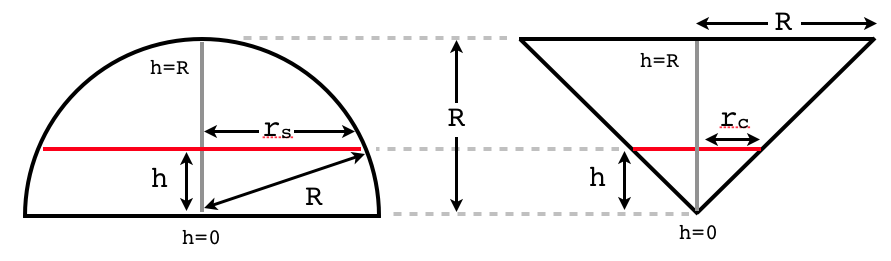
\includegraphics [scale=0.4] {sphere_cone.png} \end{center}

Now invert the cone, so that its tip is on the plane and the fattest part is farthest away.  

What Archimedes found is that for \emph{any} cross-section parallel to the $xy$-plane, at some height $h$, the slices have the property that the area of the sphere's cross-section plus the area of the cone's cross-section is a constant.  Furthermore, together they equal $\pi R^2$, the area of the cross-section of a cylinder with radius.

Pythagoras gives us the radius of the cross-section of the sphere (which is a circle) at height $h$ from the $xy$-plane as 
\[ r_s^2 = R^2 - h^2 \]

Since the cone has total height and radius both equal to $R$, and since it's inverted, at any height $h$, the radius at that height is equal to $h$

\[ r_c^2 = h^2 \]

Addition of the areas of the two cross-sections gives

\[ \pi r_s^2 + \pi r_c^2 =  \pi (R^2 - h^2) + \pi (h^2) = \pi R^2 \]

which is equal to the area of the cross-section of a cylinder with radius $R$.  

When we add up all the slices from bottom to top, since the cross-sections add  to $\pi R^2$ at any height, the total of all the cross-sections, which are volumes, add up too.

We conclude that \textbf{hemisphere plus cone equals cylinder}.  

Since the volumes of the cylinder and cone are $\pi R^3$ and $\pi R^3/3$, respectively, the volume of the hemisphere is the difference, and the volume of the sphere is twice that, namely $4/3 \pi R^3$.

\subsection*{Method of disks}
Consider a function $y = f(x)$, and imagine that we rotate the graph of the function around the $x$-axis.  The rotational symmetry allows us to calculate the volume as a single integral.

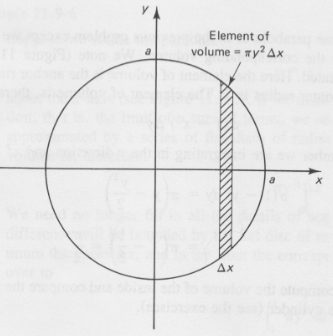
\includegraphics [scale=0.6] {sphere_vol1.png} 

The method is to "slice" the volume using slices perpendicular to the $x$-axis.  These cross-sections are circles, because of the rotation.  Every slice has volume equal to the area of that slice, $\pi y^2$, times the width $dx$, so the total volume is obtained by adding up all of the slices:
\[ V = \int  \pi y^2 \ dx \]

Our specific problem is to obtain a sphere, which we get by rotating the top half of the graph of a circle
\[ f(x) = + \sqrt{R^2 - x^2} \]

The bounds are $x = -R \rightarrow R$.  So the integral is just
\[ V = \pi \int_{-R}^R (R^2 - x^2) \ dx \]
It makes it slightly easier to notice at this point that that $R^2 - x^2$ is an even function of $x$ so 
\[ \pi \int_{-R}^R (R^2 - x^2) \ dx =  2 \pi \int_{0}^R (R^2 - x^2) \ dx \] 
We integrate from $[0,R]$ and then multiply by $2$.

\[ = 2 \pi \ [ \ (R^2x - \frac{x^3}{3}) \bigg |_{0}^{R} \ ] \]
\[ = 2 \pi \ [ \ R^3 - \frac{1}{3}R^3 \ ] \  = \frac{4}{3}\pi R^3\]

\subsection*{Method of shells}
The third approach is the method of shells.  Here is a picture of what we're doing, from Hamming's Calculus text.  The notation is different but the idea is the same.

We'll work with the hemisphere, above the $xy$-plane.

Let's divide the sphere up into concentric cylinders or shells, and let $r$ vary from $0 \to R$.  

\begin{center} 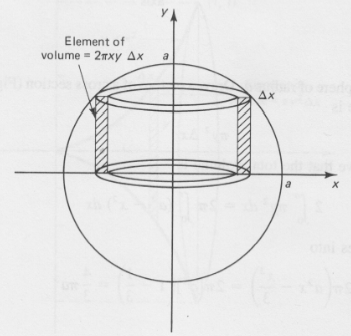
\includegraphics [scale=0.6] {sphere_vol2.png} \end{center}

The circumference of the shell at each point is 
\[ C = 2 \pi r \]
and the height of each is 
\[ h = \sqrt{R^2 - r^2} \]
The volume of each very thin cylinder is the product
\[ dV = Ch \ dr = 2 \pi r \sqrt{R^2 - r^2} \ dr \]
and we want to integrate this over the interval $[0,R]$:
\[ V = 2 \pi \int_{r=0}^{r=R} r \sqrt{R^2 - r^2} \ dr \]
\[ =  2 \pi \ [  -\frac{1}{3}\pi (R^2 - r^2)^{3/2} \ ] \  \bigg|_0^R \]
\[ =  2 \pi \ [ -\frac{1}{3}\pi \ [ \ - (R^2)^{3/2} \ ] \]
\[ = \frac{2}{3} \pi R^3 \]

Multiply by two to obtain the total volume.

\subsection*{Double integral}

We now move to multi-variable calculus, and consider the sphere as a function $f(x,y)$ of points in the $xy$-plane.  The graph of this function is plotted on the $z$-axis, above the points.  We consider one octant of the hemisphere, the part where all three of $x,y,z > 0$.  The equation is

\[ R^2 = x^2 + y^2 + z^2 \]
\[ z = f(x,y) = \sqrt{R^2 - x^2 - y^2} \]

The "shadow" of the sphere is a quadrant of the circle of radius $R$ (since $z=0$ in the $xy$-plane).  For each little area element $dA$ inside the shadow, we find the distance up to the graph of the function as $f(x,y)$.

\begin{center} 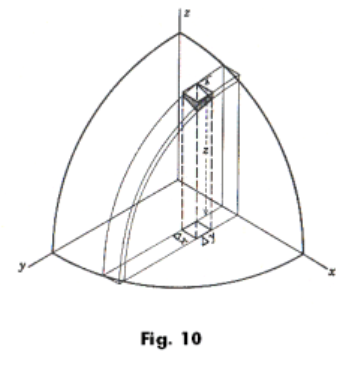
\includegraphics [scale=0.6] {sphere_double_int.png} \end{center}

Suppose we try using Cartesian coordinates, and integrate first with respect to $y$ and then with respect to $x$.  The volume is this double integral
\[ V = \int_{x=0}^{x=R} \int_{y=0}^{\sqrt{R^2-x^2}}  \sqrt{R^2 - x^2 - y^2} \ dy \ dx \]

This looks rather forbidding, but it won't be too bad.  Let us first, for the moment, substitute $a = \sqrt{R^2-x^2}$ and keep in mind that this is a constant for the inner integral.  So that part is now
\[ \int_{0}^{a} \sqrt{a^2 - y^2} \ dy \]
(We looked at this integral in the section on \hyperref[sec:Cosine_squared]{\textbf{cosine squared}}).

A little investigation reveals that the right approach to this is a trig substitution, namely 
\[ y = a \sin \theta \]
\[ dy = a \cos \theta \ d \theta \]

We will have

\[ \int \sqrt{a^2 - a^2 \sin^2 \theta} \ a \cos \theta \ d \theta \]
\[ = a^2 \int \sqrt{1 - \sin^2 \theta} \cos \theta \ d \theta \]
\[ = a^2 \int \cos^2 \theta \ d \theta \]

The crucial thing is to change the limits.  We need to find the value of $\theta$ at the old limits for $y$, namely

\[ y = 0, \ \ 0 = a \sin \theta, \ \ \theta = 0 \]
\[ y = a, \ \ a = a \sin \theta, \ \ \theta = \frac{\pi}{2} \]

So
\[ a^2 \int_0^{\pi/2} \cos^2 \theta \ d \theta \]
We've done cosine-squared many times by now.  We use the double-angle version:
\[ = a^2 \int_0^{\pi/2} \frac{1}{2}(1 + \cos 2 \theta) \ d \theta \]
\[ = a^2 \ \frac{1}{2} \ (\theta + \frac{1}{2} \sin 2 \theta) \ \bigg |_0^{\pi/2} \]
Almost everything is zero
\[ = \frac{a^2}{2} (\frac{\pi}{2} + 0 - 0 - 0) \]
\[ = a^2 \frac{\pi}{4} = (R^2-x^2) \frac{\pi}{4} \]

The outer integral is
\[ \int_{x=0}^{x=R} (R^2-x^2) \frac{\pi}{4} \ dx \]
\[ = \frac{\pi}{4} (R^2x - \frac{1}{3}x^3) \ \bigg |_0^R \]
\[ = \frac{\pi}{4} \ \frac{2}{3}R^3 = \frac{1}{6}\pi R^3 \]

Recall that this is for one octant, so for the whole sphere we multiply by $8$ and obtain:
\[ V = \frac{8}{6}\pi R^3 = \frac{4}{3}\pi R^3 \]

An easier approach would be to use polar coordinates.  We had
\[ R^2 = x^2 + y^2 + z^2 \]
\[ z = f(x,y) = \sqrt{R^2 - x^2 - y^2} \]

We let $x^2 + y^2 = r^2$ and remember that the area element in polar coordinates adds a factor of $r$ (from Jacobian):
\[ V = \iint \sqrt{R^2 - r^2} \ r \ dr \ d \theta \]
The integrals are independent.  So just do the outer one first
\[ = 2 \pi \int_0^R  \sqrt{R^2 - r^2} \ r \ dr  \]
\[ = 2 \pi \ [ \ - \frac{1}{3} (R^2 - r^2)^{3/2} \ ] \bigg |_0^R \]
\[ = \frac{2}{3} \pi R^3 \]
and since we did the volume above the $xy$-plane, we need to multiply by $2$ for the final answer.

\subsection*{Triple integral}
For the triple integral, we are integrating the volume element over the entire range of values inside the sphere.

\[ V = \iiint dV \]

We can do this integral relatively easily in both cylindrical and spherical coordinates.  For completeness, I'm going to try it in Cartesian coordinates as well.

Consider the one-eighth of the sphere that has $x>0,y>0,z>0$.

Let's work from the outside in.  We will do $x$ last.  The limits on $x$ are $x=0 \rightarrow R$.  Simple enough.  The shadow of the sphere in the $xy$-plane is a circle with radius $R$ and so the limits on $y$ are $y=0 \rightarrow \sqrt{R^2-x^2}$.

And then, naturally enough, the limits on $z$ are $z=0 \rightarrow \sqrt{R^2 - x^2 - y^2}$.

So our integral is

\[ \int_{x=0}^{R} \int_{y=0}^{\sqrt{R^2-x^2}} \int_{z=0}^{\sqrt{R^2 - x^2 - y^2}} \ dz \ dy \ dx \]

The inner integral is trivial.  The middle integral is then
\[ \int_{y=0}^{\sqrt{R^2-x^2}} \sqrt{R^2 - x^2 - y^2} \ dy \]

This is exactly the integral we solved above.  Setting $a^2 = R^2 - x^2$, the integral is of the form
\[ \int \sqrt{a^2 - y^2} \ dy \]

If you look it up, you might find an answer like this:
\[ \frac{a^2}{2} \sin^{-1} \frac{y}{a} + \frac{y \sqrt{a^2-y^2}}{2} \]
which at first sight looks much different than the solution we showed above.  There are two reasons why it is so different.  

The first is that there are two different but equivalent results for the integral of cosine squared (or sine squared).  And second, in this version, rather than stay with $\theta$ or $t$ from the trig substitution, we have gone back to the original variable.

Plugging in the upper limit $y= \sqrt{R^2-x^2}$ we obtain
\[ \frac{R^2 - x^2}{2} \sin^{-1} \frac{\sqrt{R^2-x^2}}{\sqrt{R^2-x^2}} + \frac{\sqrt{R^2-x^2} \sqrt{R^2-x^2 - (R^2-x^2)}}{2} \]

Luckily, the second term is zero.  And since $\pi/2 =  \sin^{-1} (1)$, for this part we have just

\[ = \frac{R^2 - x^2}{2} \cdot \frac{\pi}{2} \]

At the lower limit ($y=0$), the first term includes $\sin^{-1} (0)$, which equals zero, and the second term has a factor of $y$, so the whole thing is just zero.

Finally, we come to the outer integral, which is
\[ \frac{\pi}{4} \int_0^R R^2 - x^2 \ dx \]
\[ = \frac{\pi}{4} \cdot \frac{2}{3} R^3 \]
\[ = \frac{\pi}{6} R^3 \]

Since there are eight such volumes in the whole sphere, we obtain the familiar answer.

\subsection*{Triple integral in cylindrical coordinates}
 
The equation of the sphere in Cartesian coordinates is:

\[ R^2 = x^2 + y^2 + z^2 \]

Converting to polar coordinates we have 

\[ r^2 = x^2 + y^2 \]
\[ R^2 = z^2 + r^2 \]
\[ z = \sqrt{R^2 - r^2} \]

Recall that the area element in polar coordinates is $dA = r \ dr \ d \theta$.

If we integrate first with respect to $z$ we have
\[ \int \int \int dz \ r \ dr \ d \theta \]

The limits on $r$ and $\theta$ are as usual:
\[ \int_0^{2\pi} \int_0^R \int dz \ r \ dr \ d \theta \]

In particular, we integrate over the entire shadow of the sphere on the $xy$-plane.  Now, for each value of $r$ and $\theta$ we must find the limits on $z$.  From above, we get

\[ \int_0^{2\pi} \int_0^R \int_{-\sqrt{R^2 - r^2}}^{\sqrt{R^2 - r^2}} dz \ r \ dr \ d \theta \]

The inner integral is just

\[ z  \ \bigg |_{-\sqrt{R^2 - r^2}}^{\sqrt{R^2 - r^2}} = 2(\sqrt{R^2 - r^2}) \]

So the middle integral is then
\[ \int_0^R 2(\sqrt{R^2 - r^2}) \ r \ dr \]
\[ = -\frac{2}{3}(R^2 - r^2)^{3/2}  \ \bigg |_0^R = \frac{2}{3} R^3 \]

The outer integral is trivial
\[ \int_0^{2\pi} \frac{2}{3} R^3 \ d \theta = \frac{4}{3} \pi R^3  \]

\subsection*{Triple integral in spherical coordinates}

Here is the figure from \emph{How to Ace Calculus}
\begin{center} 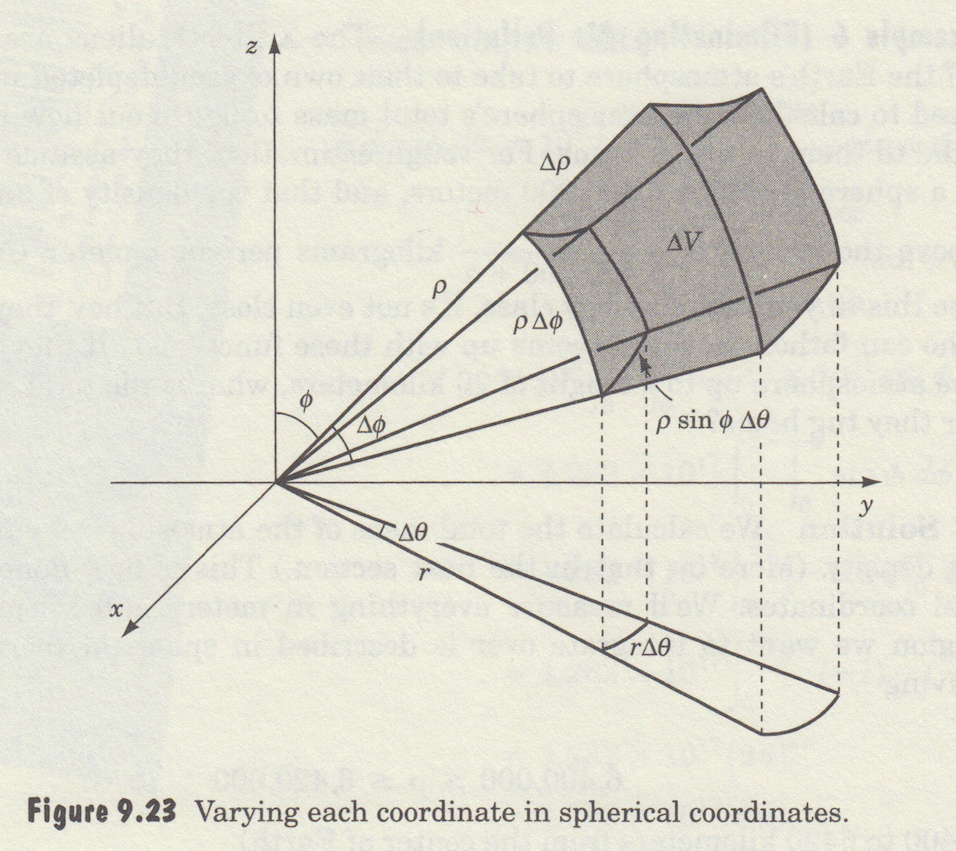
\includegraphics [scale=0.25] {sphcoord.png} \end{center}

In spherical coordinates, we see that the volume element is 
\[ dV = \rho^2 \sin \phi \ d \rho \ d \phi \ d \theta \]

And having used that, our work is essentially done.  We just set up the integral
\[ \int_0^{2\pi} \int_0^{\pi} \int_0^R \rho^2 \sin \phi \ d \rho \ d \phi \ d \theta \]

The peculiarity of this is that the limits on $\rho$ do not depend on the angles $\phi$ and $\theta$.  So now the inner integral is just 
\[ = \int_0^R \rho^2 \sin \phi \ d \rho = \frac{1}{3}R^3 \sin \phi \]

And the term $R^3/3$ is a constant.  So we put that aside and evaluate the middle integral
\[ \int_0^{\pi} \sin \phi \ d \phi \]
\[ = - \cos \phi \ \bigg |_0^{\pi} = - (- 2) = 2\]

So in the end we have 
\[ 2 \pi \cdot 2 \cdot \frac{1}{3}R^3 = \frac{4}{3} \pi R^3 \]

\subsection*{Deriving the formula we used}
Up above in the first section of volume integrals (Cartesian coordinates) we used this formula
\[ \int \sqrt{a^2 - y^2} \ dy = \frac{a^2}{2} \sin^{-1} \frac{y}{a} + \frac{y \sqrt{a^2-y^2}}{2} \]

Let me re-write it in a more familiar but equivalent form.  We use a simple trig substitution.
\[ \frac{x}{a} = \sin t \]
\[ x = a \ \sin t \]
\[ dx = a \ \cos t \ dt \]
Using Pythagoras
\[ \sqrt{a^2 - x^2} = a \cos t \]
Substituting
\[ \int \sqrt{a^2 - x^2} \ dx \]
\[ = \int  a \cos t \ a \cos t \ dt \] 
\[ = a^2 \int  \cos^2 t \ dt \]
An old friend!  I'm not going to work this one out from scratch, we've seen it several times.  One of the equivalent forms for this integral is

\[ \int \cos^2 t \ dt = \frac{1}{2}(t + \sin t \cos t) \]
Picking up the outside factor of $a^2$ and substituting we obtain

\[ = a^2 \ \frac{1}{2} (\sin^{-1}\frac{x}{a} + \frac{x}{a} \cdot \frac{\sqrt{a^2-x^2}}{a} ) \]
\[ = \frac{a^2}{2} \sin^{-1} \frac{x}{a} + \frac{x \sqrt{a^2-x^2}}{2} \]

\end{document}  